\section{Preprocessing}
At this stage, the EMG signals should be recorded by the armband and the hand movements by the data glove to create a database containing the type of gestures and the corresponding signal.  Recorded signals are raw data and require preprocessing to be used for network training and testing. The preprocessing phase includes filtering, normalizing, windowing, labeling the data, and finally converting it into three subsets: train, validation, and test [26,27].

The UC2018 database is used to avoid prolonging the research path. This data set is obtained from two EMG sensors (Myo) with a subject that performs eight distinct hand gestures. There are a total of 110 repetitions of each class of gesture obtained across five recording sessions. Each armband contains eight sensors that record data at a frequency of 200 Hz. Since the sampling time is 2 seconds, the dimension of the data is 16×400. Some preprocessing steps have been performed in this database, including removing municipal electricity and heartbeat noise [28]. Figure 1 shows eight movements related to the signals of this database.

\begin{figure}
    \centering
    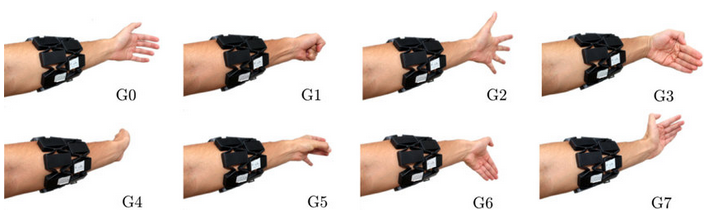
\includegraphics[scale=0.49]{figures/gestures.png}
    \caption{\centering
    UC2018 DualMyo dataset gestures: (G0) rest, (G1) closed fist, (G2) open hand, (G3) wave in, (G4) wave out, (G5) double-tap, (G6) hand down, (G7) hand up}
    \label{fig:gestures}
\end{figure}

Although the noise removal operation performed on the data set, the data is still not suitable for model input. The signals are long, and the amount of data to train the deep network is not sufficient. In order to solve this problem, first, the signals are stacked, and then using the windowing technique data is split into signals with less length. For this purpose, the length of each window and the amount of overlap must be specified. In this study, the window size is 125 milliseconds for real-time and 1 second for offline usage without overlap. The last 15 and 50 data of each sample is used for labeling, respectively, and the label with the most repetition is selected as the sample label. 14080 signals with dimensions of $25 \times 16$ and $200 \times 16$ were obtained, which are both the right size and sufficient number. The signal range is -128 to 128. In order to increase the speed of convergence of the network and also stabilize the network and preventing from gradient exploding, it is necessary to normalize the input data. For this reason, the MinMax is used and all data are divided by the maximum value, 128 so that the data are in the range of -1 and +1. The data were then randomly divided into three train, test, and validation groups, with a ratio of 70\%, 15\%, and 15\%  so that the test data is completely unseen.